% Options for packages loaded elsewhere
\PassOptionsToPackage{unicode}{hyperref}
\PassOptionsToPackage{hyphens}{url}
%
\documentclass[
]{article}
\usepackage{amsmath,amssymb}
\usepackage{lmodern}
\usepackage{ifxetex,ifluatex}
\ifnum 0\ifxetex 1\fi\ifluatex 1\fi=0 % if pdftex
  \usepackage[T1]{fontenc}
  \usepackage[utf8]{inputenc}
  \usepackage{textcomp} % provide euro and other symbols
\else % if luatex or xetex
  \usepackage{unicode-math}
  \defaultfontfeatures{Scale=MatchLowercase}
  \defaultfontfeatures[\rmfamily]{Ligatures=TeX,Scale=1}
\fi
% Use upquote if available, for straight quotes in verbatim environments
\IfFileExists{upquote.sty}{\usepackage{upquote}}{}
\IfFileExists{microtype.sty}{% use microtype if available
  \usepackage[]{microtype}
  \UseMicrotypeSet[protrusion]{basicmath} % disable protrusion for tt fonts
}{}
\makeatletter
\@ifundefined{KOMAClassName}{% if non-KOMA class
  \IfFileExists{parskip.sty}{%
    \usepackage{parskip}
  }{% else
    \setlength{\parindent}{0pt}
    \setlength{\parskip}{6pt plus 2pt minus 1pt}}
}{% if KOMA class
  \KOMAoptions{parskip=half}}
\makeatother
\usepackage{xcolor}
\IfFileExists{xurl.sty}{\usepackage{xurl}}{} % add URL line breaks if available
\IfFileExists{bookmark.sty}{\usepackage{bookmark}}{\usepackage{hyperref}}
\hypersetup{
  pdftitle={Supplement to The Evolving Roles of Partisanship and Vulnerability in the COVID-19 Pandemic},
  hidelinks,
  pdfcreator={LaTeX via pandoc}}
\urlstyle{same} % disable monospaced font for URLs
\usepackage[margin=1in]{geometry}
\usepackage{graphicx}
\makeatletter
\def\maxwidth{\ifdim\Gin@nat@width>\linewidth\linewidth\else\Gin@nat@width\fi}
\def\maxheight{\ifdim\Gin@nat@height>\textheight\textheight\else\Gin@nat@height\fi}
\makeatother
% Scale images if necessary, so that they will not overflow the page
% margins by default, and it is still possible to overwrite the defaults
% using explicit options in \includegraphics[width, height, ...]{}
\setkeys{Gin}{width=\maxwidth,height=\maxheight,keepaspectratio}
% Set default figure placement to htbp
\makeatletter
\def\fps@figure{htbp}
\makeatother
\setlength{\emergencystretch}{3em} % prevent overfull lines
\providecommand{\tightlist}{%
  \setlength{\itemsep}{0pt}\setlength{\parskip}{0pt}}
\setcounter{secnumdepth}{-\maxdimen} % remove section numbering
\ifluatex
  \usepackage{selnolig}  % disable illegal ligatures
\fi
\newlength{\cslhangindent}
\setlength{\cslhangindent}{1.5em}
\newlength{\csllabelwidth}
\setlength{\csllabelwidth}{3em}
\newenvironment{CSLReferences}[2] % #1 hanging-ident, #2 entry spacing
 {% don't indent paragraphs
  \setlength{\parindent}{0pt}
  % turn on hanging indent if param 1 is 1
  \ifodd #1 \everypar{\setlength{\hangindent}{\cslhangindent}}\ignorespaces\fi
  % set entry spacing
  \ifnum #2 > 0
  \setlength{\parskip}{#2\baselineskip}
  \fi
 }%
 {}
\usepackage{calc}
\newcommand{\CSLBlock}[1]{#1\hfill\break}
\newcommand{\CSLLeftMargin}[1]{\parbox[t]{\csllabelwidth}{#1}}
\newcommand{\CSLRightInline}[1]{\parbox[t]{\linewidth - \csllabelwidth}{#1}\break}
\newcommand{\CSLIndent}[1]{\hspace{\cslhangindent}#1}

\title{Supplement to The Evolving Roles of Partisanship and
Vulnerability in the COVID-19 Pandemic}
\author{}
\date{\vspace{-2.5em}}

\begin{document}
\maketitle

\hypertarget{introduction}{%
\subsection{Introduction}\label{introduction}}

These supplemental materials present a conditional auto-regressive (CAR)
Poisson model of COVID-19 county death rates in the United States. The
inclusion of a conditional auto-regressive spatial component in this
model is intended to address the question of how robust the
relationships are between observed covariates and COVID-19 death rates
given the expected correlations in rates between counties which neighbor
one another.

\hypertarget{methods}{%
\subsection{Methods}\label{methods}}

The implementation of our model is based on the Stan Case Study,
\emph{Exact Sparse CAR Models in Stan} (Joseph 2016). Spatial models
including CAR models and improvements on the Besag-York-Mollié model
have often been used in current epidemiology and disease risk mapping
applications to distinguish spatially structured effects from the
effects of observed covariates {[}Lee, Rushworth, and Sahu (2014);
Wakefield (2007); Morris et al.~(2019){]}.

To describe our model, we write the deaths observed as
\(y_1, y_2, ..., y_{2683}\) for each of the 2,683 counties which have
neighboring counties and for which all covariates were available and
hence were considered in our main manuscript. Letting \(X_i\) for \(i\)
in 1\ldots2,683 represent the vector of observed covariates for the
\(i\)th county and similarly \(P_i\) represent the population of the
\(i\)th county, we write that

\[y_i \sim \text{Poisson}(\text{exp}(X_i \beta + \phi_i + \text{log}(P_i))),\]

where \(\beta\) is a vector of the estimated coefficients for the
covariates and \(\phi_i\) is the the spatial component of the model. See
Joseph (2016) for the details of the prior distributions on \(\beta\)
and \(\phi\). This model is fit twice with data from period 2 and period
3 separately.

Given the computational complexity in fitting these models with over
2600 county observations and a large number of covariates, we opted to
only include a selection of the variables which had the highest measures
of feature importance in the LASSO and spatial linear models from our
main manuscript. In order to include parameters parsimoniously, we chose
to include parameters which appeared in the top three most important
features from the LASSO and spatial linear models for periods 2 and 3.
Since we only modeled the probability of counties being seeded during
period 1 and did not model death rates, we have only calibrated the
spatial model presented here to the deaths data from periods 2 and 3.

All analyses in these supplemental materials were conducted using R
version 4.0.2 (R Core Team 2020) and the model analyses were conducted
in the Bayesian statistical computing and modeling framework Stan using
the No-U-Turns Hamiltonian Monte Carlo Sampler (Stan Development Team
2021; Homan, Matthew D. and Gelman, Andrew 2014).

\newpage

\hypertarget{results}{%
\subsection{Results}\label{results}}

\hypertarget{parameter-estimates}{%
\subsubsection{Parameter Estimates}\label{parameter-estimates}}

We found that the results of fitting a spatial sparse CAR Poisson model
were consistent with our findings from the main analyses for periods 2
and 3.

\begin{figure}

{\centering 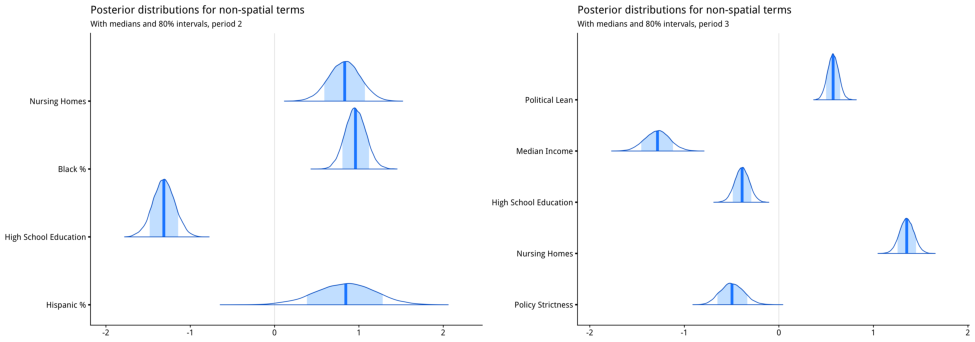
\includegraphics[width=1\linewidth,height=0.4\textheight]{supplement_files/figure-latex/unnamed-chunk-1-1} 

}

\caption{Non-spatial parameter estimates for periods 2 and 3}\label{fig:unnamed-chunk-1}
\end{figure}

These model estimates reflect the associations between county-level
covariates and COVID-19 death rates after accounting for the estimated
spatial correlation structure included in the model.

We found that higher percentages of residents in nursing homes, Black
non-Hispanic population percentages, and Hispanic population percentages
at the county level were associated with higher COVID-19 death rates
during period 2.Counties with higher high school graduation rates were
associated with having lower COVID-19 death rates in period 2 after
accounting for spatial correlations. During period 3, counties where the
population voted more Republican (positive political lean), and counties
with higher percentages of the population living in nursing homes were
associated with higher COVID-19 death rates. Counties with higher median
income, greater high school graduation rates, and policy strictness
during period 3 were found to be have lower COVID-19 death rates.

\newpage

\hypertarget{spatial-components}{%
\subsubsection{Spatial Components}\label{spatial-components}}

We present the spatial model component below visualized as
\(\text{exp}(\phi_i + \text{log}(P_i))\), the expected COVID-19 deaths
per capita in each period conditioning out the effects from covariates.

\begin{figure}

{\centering 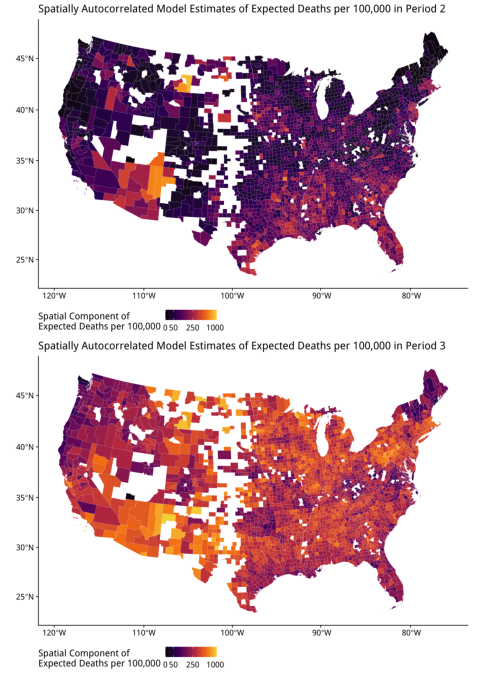
\includegraphics[width=0.8\linewidth,height=0.6\textheight]{supplement_files/figure-latex/unnamed-chunk-2-1} 

}

\caption{Spatial model component during periods 2 and 3}\label{fig:unnamed-chunk-2}
\end{figure}

Supplemental Figure 2 allows us to visualize the estimated spatial
correlation structure and how neighboring counties tend to be correlated
with one another. In essence, we expect to see that counties which have
high rates are surrounded by counties that also have high rates and
vice-versa for low rate counties.

\newpage

\hypertarget{model-convergence-diagnostics}{%
\subsubsection{Model Convergence
Diagnostics}\label{model-convergence-diagnostics}}

\begin{figure}

{\centering 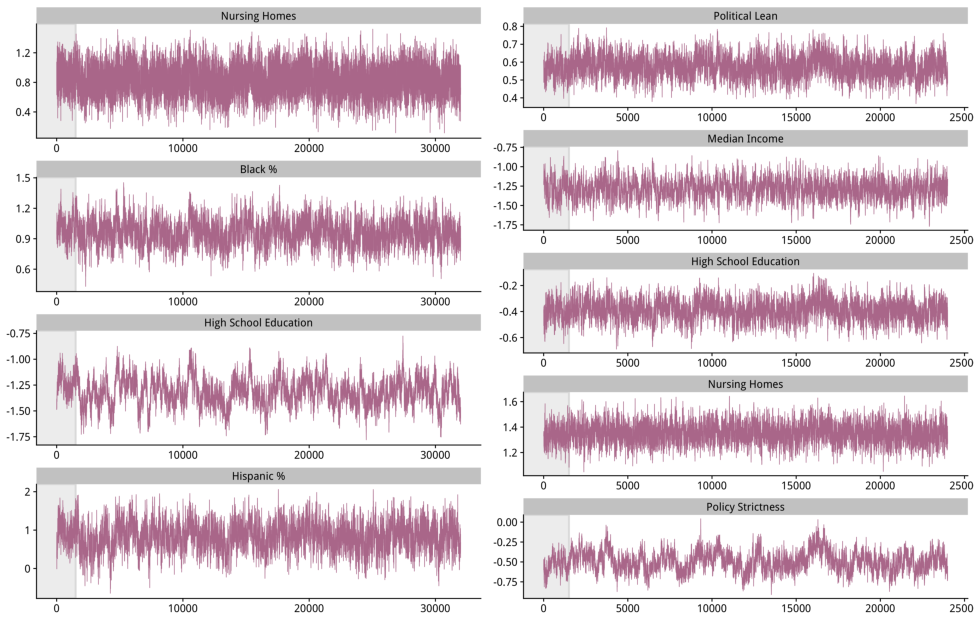
\includegraphics[width=0.6\linewidth,height=0.25\textheight]{supplement_files/figure-latex/unnamed-chunk-3-1} 

}

\caption{Traceplots for non-spatial parameters}\label{fig:unnamed-chunk-3}
\end{figure}

Contemporary advice recommends that Bayesian models should be considered
to have converged only if the Markov chains have convergence diagnostics
of \(\hat{R} < 1.05\) (Stan Development Team 2020; Vehtari et al. 2020).
In Supplemental Figure 4 we present the \(\hat{R}\) convergence
diagnostics for our non-spatial and spatial effects for both periods 2
and 3 which are all below 1.05.

\begin{figure}

{\centering 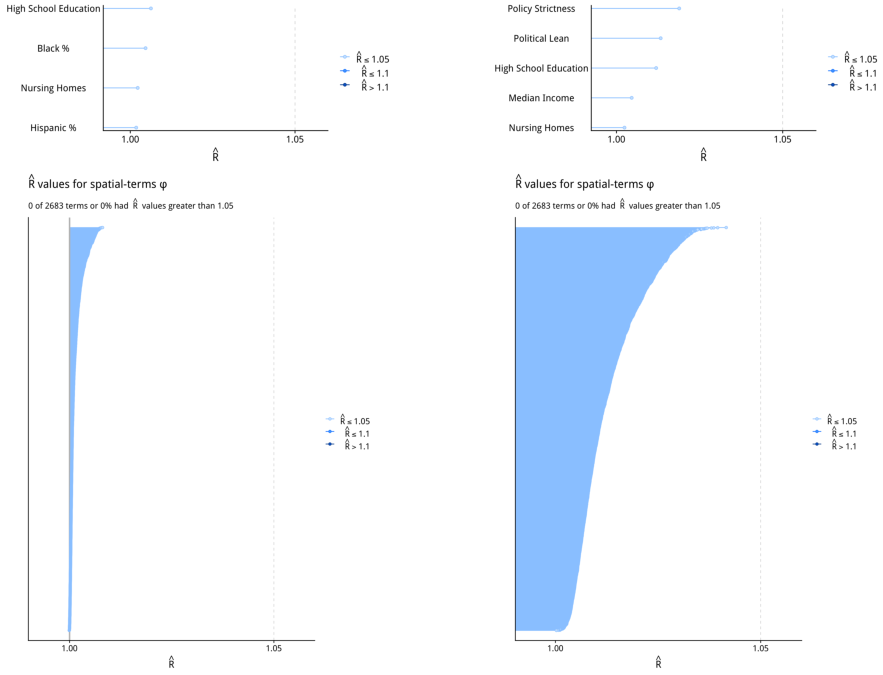
\includegraphics[width=1\linewidth,height=0.4\textheight]{supplement_files/figure-latex/unnamed-chunk-4-1} 

}

\caption{Convergence diagnostics for all parameters}\label{fig:unnamed-chunk-4}
\end{figure}

\newpage

\hypertarget{references}{%
\subsection*{References}\label{references}}
\addcontentsline{toc}{subsection}{References}

\hypertarget{refs}{}
\begin{CSLReferences}{1}{0}
\leavevmode\hypertarget{ref-homan_no-u-turn_2014}{}%
Homan, Matthew D. and Gelman, Andrew. 2014. {``The {No}-{U}-Turn
Sampler: Adaptively Setting Path Lengths in {Hamiltonian} {Monte}
{Carlo}.''} \emph{The Journal of Machine Learning Research} 15
(January). \url{https://dl.acm.org/doi/10.5555/2627435.2638586}.

\leavevmode\hypertarget{ref-exact-sparse-car}{}%
Joseph, Maxwell. 2016. \emph{{Exact Sparse CAR Models in Stan}}.
\emph{Stan Case Studies}. Vol. 3.

\leavevmode\hypertarget{ref-lee_bayesian_2014}{}%
Lee, Duncan, Alastair Rushworth, and Sujit K. Sahu. 2014. {``A
{Bayesian} Localized Conditional Autoregressive Model for Estimating the
Health Effects of Air Pollution.''} \emph{Biometrics} 70 (2): 419--29.
\url{https://doi.org/10.1111/biom.12156}.

\leavevmode\hypertarget{ref-R-base}{}%
R Core Team. 2020. \emph{R: A Language and Environment for Statistical
Computing}. Vienna, Austria: R Foundation for Statistical Computing.
\url{https://www.R-project.org/}.

\leavevmode\hypertarget{ref-rhat}{}%
Stan Development Team. 2020. \emph{Convergence and Efficiency
Diagnostics for Markov Chains, Rstan 2.12.2 Documentation}.
\url{https://mc-stan.org/rstan/reference/Rhat.html}.

\leavevmode\hypertarget{ref-Stan}{}%
---------. 2021. \emph{Stan Modeling Language Users Guide and Reference
Manual, V2.26}. \url{https://mc-stan.org}.

\leavevmode\hypertarget{ref-vehtari_rank-normalization_2020}{}%
Vehtari, Aki, Andrew Gelman, Daniel Simpson, Bob Carpenter, and
Paul-Christian Bürkner. 2020. {``Rank-Normalization, Folding, and
Localization: {An} Improved \${\textbackslash{}}Widehat\{{R}\}\$ for
Assessing Convergence of {MCMC}.''} \emph{Bayesian Analysis}, July.
\url{https://doi.org/10.1214/20-BA1221}.

\leavevmode\hypertarget{ref-wakefield_disease_2007}{}%
Wakefield, Jon. 2007. {``Disease Mapping and Spatial Regression with
Count Data.''} \emph{Biostatistics} 8 (2): 158--83.
\url{https://doi.org/10.1093/biostatistics/kxl008}.

\end{CSLReferences}

\end{document}
